\subsection {Other Systematics}
Two other sources of systematic uncertainty were assessed  by other members of the analysis team and outlined in this section.

The systematic due to the prescale, luminosity weights and trigger inefficencies in the trigger strategy was assessed using the PYTHIA sample and found to be negligible in all final distributions.

The unfolding method used was the bayesian unfolding method.
Two different uncertainties were assesed and combined in quadrature for the unfolding; one was due to model uncertainty and the other was due to the statistics in the MC sample. 
The main contribution to the model uncertainty was due to the uncertainty in the shape of the $\pt{}_3$ distribution, where $\pt{}_3$ is the highest \pt{} jet bounded by the dijet system. 
This $\pt{}_3$ distribution was varied within the JES uncertainty by weighting the events. 
The unfolding when then recalculated and the uncertainty found from the spread.
The author provided the scaling which was applied to the MC events to vary the shape of the $\pt{}_3$ distribution.
Figure \ref{GBJ2:Uncorr:pt3} shows this ratio between uncorrected data and MC with the JES uncertainty band shown in red.
For the model uncertainty, the $\pt{}_3$ distributions is allowed to vary maximally withing the JES uncertainty band.
The two blue lines on the plot shows the reweighing factors that were used to assess this model uncertainty.
\begin{figure}
\centering
\mbox{
   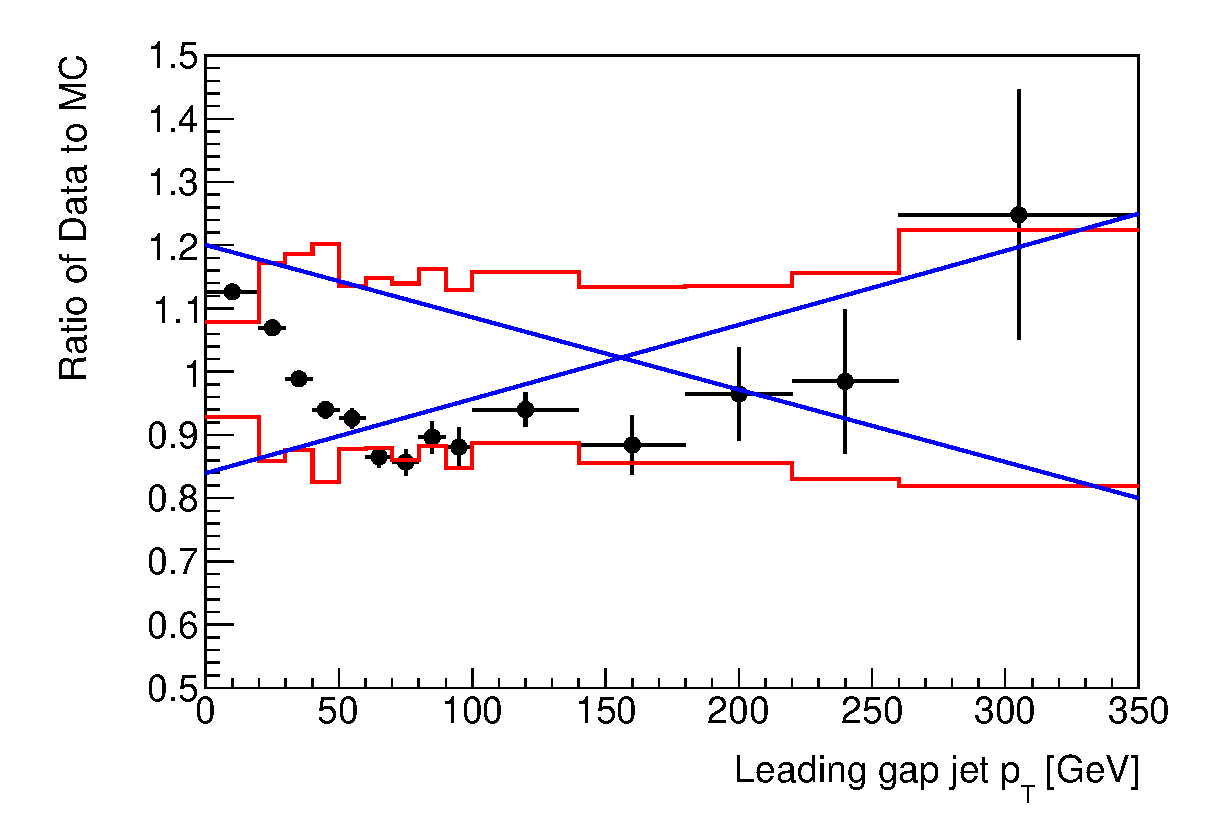
\includegraphics[width=0.8\textwidth]{figures/GBJ2/ControlPlots/Ratio___pt3.eps}
}
\caption[]{
Ratio of the \pt{} of the leading gap jet from 2010 uncorrected data to that of the reconstructed PYTHIA sample.
The red lines show the JES uncertainty bands.
\label{GBJ2:Uncorr:pt3}}
\end{figure}


\subsection{Combined Systematics}
\label{sec:GBJ2:SysComb}

The systematics studied above were combined  with the systematic uncertainties from the unfolding process and the trigger inefficencies, to produce the overall systematic uncertainty, some of which are shown in Figures \ref{GBJ2:SysComb:GapNjet} -- \ref{GBJ2:SysComb:cos2}.

Figure \ref{GBJ2:SysComb:GapNjet} shows the systematic uncertainty on (a) the gap fraction and (b) the average number of jets as a function of \dy{}
The dominant systematic is due to the JES uncertainty, while the unfolding also makes a significant contribution. 
The effect from JER is small, and the effect due to $\phi$ resolution is zero.


Figure \ref{GBJ2:SysComb:dphi23} shows the systematic uncertainty on the differential cross section, \dphiDist, for (a) inclusive events and (b) gap events.
The dominant systematics are again the JES uncertainty and the unfolding, while the effect from the $\phi$ resolution and the JER are small.

Figure \ref{GBJ2:SysComb:cos2} shows the systematic uncertainty on the average \costwodphi{} for (a) inclusive events and (b) gap events as a function of \dy{}.
For the inclusive distribution there is no overall dominant systematic. 
At low \dy{}, the uncertainty from the $\phi$ resolution is large, with JES and unfolding uncertainties also contributing.
At large \dy{}, the uncertainty is dominated by the JES and unfolding.
For the gap distribution, again at low \dy{} the $\phi$ resolution is the dominant systematic and at larger \dy{} all the uncertainties have an effect. 

\begin{figure}
\centering
\mbox{
              \subfigure[]{\epsfig{figure=figures/GBJ2/FinalPlots/GapFraction_dyBins.systematics.eps,width=0.5\textwidth}}\quad
              \subfigure[]{\epsfig{figure=figures/GBJ2/FinalPlots/nGapJets_dyBins.systematics.eps,width=0.5\textwidth}}\quad
                              }
\caption[]{
The combined systematics on (a) the gap fraction and (b) the average number of jets in the dijet rapidity region as a function of \dy{}.
The combined systematics are from unfolding, JES uncertainty, JER and jet $\phi$ resolution.
\label{GBJ2:SysComb:GapNjet}}
\end{figure}
\begin{figure}
\centering
\mbox{
              \subfigure[]{\epsfig{figure=figures/GBJ2/FinalPlots/CrossSection.Inclusive.DPhiBins.2dY3.systematics.eps,width=0.5\textwidth}}\quad
              \subfigure[]{\epsfig{figure=figures/GBJ2/FinalPlots/CrossSection.Gap.DPhiBins.2dY3.systematics.eps,width=0.5\textwidth}}\quad
                              }
\caption[]{
The combined systematics on the differential cross section as a function of \dphi{}  for (a) inclusive events and (b) gap events for the \dy{} range 2--3.
The combined systematics are from unfolding, JES uncertainty, JER and jet $\phi$ resolution.
\label{GBJ2:SysComb:dphi23}}
\end{figure}


\begin{figure}
\centering
\mbox{
              \subfigure[]{\epsfig{figure=figures/GBJ2/FinalPlots/CosTwoDeltaPhiInclusive_dyBins.systematics.eps,width=0.5\textwidth}}\quad
              \subfigure[]{\epsfig{figure=figures/GBJ2/FinalPlots/CosTwoDeltaPhiGap_dyBins.systematics.eps,width=0.5\textwidth}}\quad
                              }
\caption[]{
The combined systematics on the average \costwodphi{} as a function of \dy{}  for (a) inclusive events and (b) gap events.
The combined systematics are from unfolding, JES uncertainty, JER and jet $\phi$ resolution.
\label{GBJ2:SysComb:cos2}}
\end{figure}

